\chapter{Marco Metodológico}

\par En este capítulo se describirá la secuencia del algoritmo desarrollado para el cálculo de las variables por sección en el horno, haciendo referencia a los métodos y ecuaciones antes descritos. Finalizando con la descripción de la interfaz gráfica diseñada para introducir y mostrar los datos y resultados del simulador.

\section{Algoritmo}

\par El diagrama ilustrado en la Figura \ref{fig:diagrama-algo}, permite visualizar la secuencia del algoritmo y sera detallado en las subsecciones consiguientes.

\begin{figure}[hbt]
\begin{center}
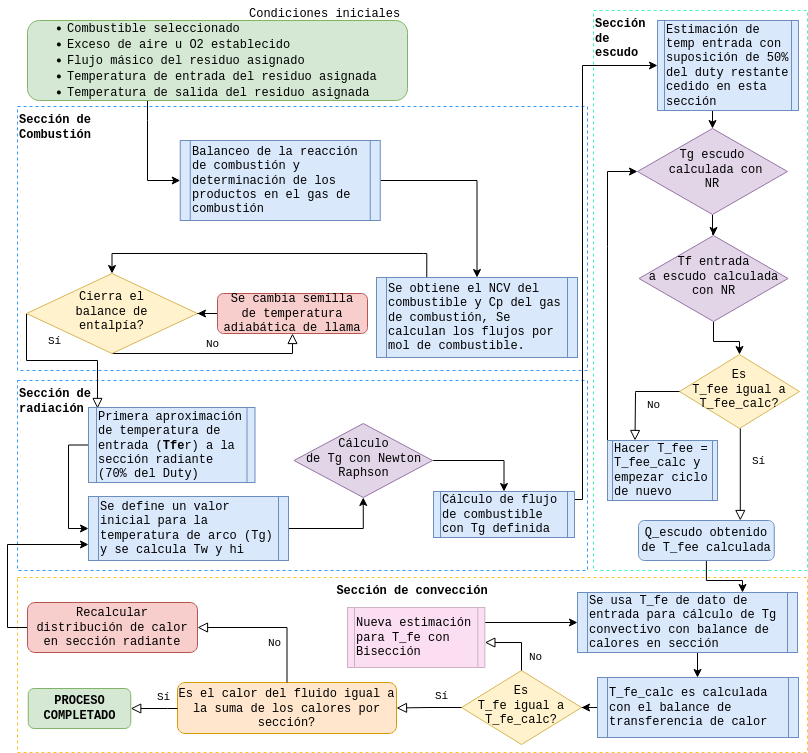
\includegraphics[scale=0.45]{images/diagrama-algo}
\caption[Diagrama de algoritmo]{Diagrama descriptivo del algoritmo desarrollo para el simulador.}
\label{fig:diagrama-algo}
\end{center}
\end{figure}

\par Datos iniciales:\\
- Propiedades del fluido, flujo volumétrico, gravedad especifica, calor especifico, conductividad térmica, viscosidad y temperatura, para la entrada y salida.\\
- Composición y temperatura del combustible.\\
- Composición, humedad relativa y temperatura del aire atmosférico.\\
- Configuración y dimensiones del horno.\\
- Propiedades y dimensiones de los tubos y aletas.

\subsection{Ciclo externo}

\par Este ciclo se encarga de recibir todos los parámetros de entrada y correr cada una de las siguientes subsecciones como funciones, es donde se define la distribución de calor entre las secciones del horno y varia este valor para alcanzar la tolerancia deseada con un método Newton Rapshon aplicado a la siguiente ecuación.

\begin{equation}
\label{eq:ciclo_externo}
\frac{(Q_{residuo} - Q_{calc})}{Q_{calc}} \approx 0
\end{equation}
\par Donde:\\
$Q_{residuo} = m_{residuo} * C_{p_residuo} * {\Delta}T_{residuo}$ \\
$Q_{calc} = Q_{RAD} + Q_{ESC} + Q_{CONV}$ \\
$Q$ = Calor o $Duty$. \\

\par Lo que se traduce en que el calor absorbido por el residuo debe ser igual al calor suministrado en cada una de las secciones del horno.

\par El valor inicial de distribución radiante esta definido en 64\% y esta converge para el rango de temperaturas permitido en la interfaz del simulador. En las siguientes subsecciones se detallan las ecuaciones para cada etapa del horno.

\subsection{Combustión}

\par Esta sección del algoritmo esta encargada de calcular toda la energía que entra al horno a través de un balance de masa y energía sobre el combustible.
\par Las propiedades del combustible son calculadas con la composición del gas ingresada.
\par En el simulador se programaron las funciones de calor especifico, viscosidad, conductividad con dependencia en la temperatura y con datos tomados del NIST\cite{nist} y las tablas de Borgnakke y Sonntag\cite{bib:vanwylen}
\par Finalmente se calcula la relación aire/combustible, la temperatura adiabática de llama y el poder calorífico del combustible NCV.

\subsubsection{Exceso de aire y exceso de \ac{o2}}
\par En caso de introducir el exceso de aire el cálculo esta programado de forma directa, si la variable introducida es el exceso de \ac{o2}, el simulador procederá a estimar este valor con el método aproximado de Newton Rapshon.

\subsection{Radiación}
\par Tres variables quedan por determinar en esta sección $Q_{RAD}$, la temperatura de entrada del fluido a la zona $T_{fer}$ radiante y la temperatura efectiva del gas $T_g$.

\par \textbf{Suposición A}
\par Se supone una distribución inicial del calor (Duty) del horno como 70\% en la zona radiante y el 30\% entre la zona escudo y zona convectiva, en consecuencia:
\begin{equation*} Q_{RAD} = 0.7 * Duty \end{equation*}
\par El $Q_{RAD}$ supuesto corresponde al valor inicial de un procedimiento de ensayo y error que cierra con al obtener un Duty calculado ($Q_{RAD} + Q_{ESC} + Q_{CONV}$) igual al Duty especificado. A partir de $Q_{RAD}$ se pueden estimar las siguientes variables:
\begin{itemize}
\item De la ecuación (\ref{eq:rad-fluid}) se obtiene la temperatura de entrada del fluido a la zona radiante $T_{fer}$ y la temperatura de mezcla $T_b$.
\item Conocida el área de los tubos se obtiene $Flux_R = Q_{RAD} /At$.
\item De la ecuación (\ref{eq:hi}) se obtiene el coeficiente de película $h_i$. Los números de Re y Pr se calculan a $T_b$.
\item De la ecuación (\ref{eq:tw}) se obtiene la temperatura de pared del tubo $T_w$.
\item Con $T_w$ calculada se recalcula $h_i$, incluyendo la corrección por viscosidad y $T_w$.
\end{itemize}
\par Todos los valores calculados dependen del supuesto A, el  posterior ajuste de QR modifica estos valores.
\par \textbf{Suposición B}
\par Seguidamente se estima, una temperatura $T_g$, para calcular los parámetros de la ecuación de radiación $\alpha$ y F.
\par Finalmente mediante la ecuación (\ref{eq:rad-tgr}) se calcula la Temperatura Efectiva del gas, $T_g$ y mediante la ecuación (\ref{eq:rad-comp}) el consumo  de combustible correspondiente a la suposición A.
\par Un recalculo del coeficiente de película, incluyendo la corrección de viscosidad, y de los parámetros de radiación $\alpha$ y F utilizando substituciones sucesivas de las temperaturas $T_g$ y $T_w$ calculadas, para así cerrar la suposición B, completan el cálculo inicial de la zona radiante.

\subsection{Escudo}
\par De la zona escudo se conocen tres variables, la temperatura de salida del fluido $T_{fer}$, la temperatura de entrada del gas de combustión $T_{gr}$ = $T_g$ y la cantidad de calor por radiación que escapa hacia la zona escudo $Q_{radEsc}$. Son incógnitas la temperatura de salida del gas $T_{ge}$, la temperatura de entrada del fluido $T_{fee}$ y el calor transferido $Q_{ESC}$.
\par \textbf{Suposición C}
\par Suponer la temperatura de entrada del fluido de la zona escudo $T_{fee}$. Recurriendo nuevamente al Duty especificado. El 30\% del Duty fue asumido que se transfieren en la zona escudo y la zona convectiva, si consideramos que en el escudo se absorbe el calor por radiación que escapa de la zona radiante lo que en cierta forma compensa la menor área de transferencia en comparación con la zona convectiva, como una razonable aproximación se suponer que:
\begin{equation*} Q_{ESC} \approx Q_{CONV} \approx 0.15 * Duty \end{equation*}
\begin{equation*} Q_{ESC_{sup}} = 0.15 * Duty \end{equation*}
\par Esto conlleva a un valor inicial para el ensayo-error de $T_{fee}$ = ($T_{fer}$ +$T_{fe}$)/2. 

\begin{itemize}
\item A partir de la ecuación (\ref{eq:esc}) calcular la temperatura de salida del gas $T_{ge}$.
\item Calcular la temperatura de mezcla del gas $T_{gb}$ y del fluido $T_{fb}$.
\item Calcular LMTD mediante la ecuación (\ref{eq:qesc-lmtd}).
\item Calcular ho, hr, hi mediante las ecuaciones (\ref{eq:hi}), (\ref{eq:ho}) y (\ref{eq:hr}).
\item Calcular Uo.
\item Calcular $Q_{ESC}$ a partir de la ecuación (\ref{eq:tesc}).
\item Calcular $T_{fee}$ a partir de la ecuación (\ref{eq:lmtd}).
\item Comparar $T_{fee}$ calculada con $T_{fee}$ supuesta.
\end{itemize}
\par Si $|(T_{fee_c} - T_{fee_s})/T_{fee_s}| > error$, se hace $T_{fee_s} = T_{fee_c}$ y $Q_{ESC_{sup}} = Q_{ESC_{calc}}$ y se regresa al primer punto.
\par Si $|(T_{fee_c} - T_{fee_s})/T_{fee_s} | < error$, se da por cerrado el cálculo de la zona de escudo. Al final del proceso $(Q_{ESC_{calc}} - Q_{ESC_{sup}})/ Q_{ESC_{sup}}$ debe estar en un valor cercano a cero.

\subsection{Convección}
\par En la zona conectiva las variables conocidas provenientes del cálculo de la zona Radiante y Escudo son la temperatura del gas a la entrada  $T_{ge}$ y la temperatura de salida del fluido $T_{fee}$. Adicionalmente se conoce, por ser especificada, la temperatura de entrada del fluido a la zona convectiva $T_{fe}$.
\par \textbf{Suposición D}
\par Suponer el valor de $T_{fe}$ igual al especificado y: 
\begin{itemize}
\item Calcular la temperatura de salida del gas $T_{gc}$ y el calor transferido $Q_{CONV}$ correspondiente mediante la ecuación (\ref{eq:conv}).
\item Calcular temperatura de mezcla del gas y del fluido.
\item Calcular LMTD.
\item Calcular Uo, según las ecuaciones descritas para tubos con aleta.
\item Calcular $Q_{CONV_{calc}}$ a partir de la ecuación (\ref{eq:qconv}).
\end{itemize}
\par Si $|(Q_{CONV_{calc}} - Q_{CONV_{sup}})/Q_{CONV_{sup}} | > error$ se recalcular la temperatura de entrada del fluido $T_{fe}$ y se vuelve al punto inicial.
\par Si $|(Q_{CONV_{calc}} - Q_{CONV_{sup}})/Q_{CONV_{sup}} | < error$, se cierra el cálculo en la zona convectiva.
\par Las variables calculadas al finalizar el procedimiento son  $Q_{CONV}, T_{fe} y T_{ge}$.

\subsection{Cierre del cálculo del horno}
\par A este nivel de avance se han calculado $Q_{RAD}, Q_{ESC}, Q_{CONV}$ y todas las temperaturas excepto la temperatura del fluido a la salida del horno $T_{fs}$, la cual se ha mantenido igual a la especificada. El control del proceso de simulación vuelve al ciclo externo y dos comprobaciones con los valores calculados son posibles:
\par Es la temperatura de entrada $T_{fe}$ calculada $>, <$ ó = a la $T_{fe}$ especificada.
\par Es $Q_{RAD} + Q_{ESC} + Q_{CONV} >, <$ ó = al Duty especificado.
 
\par Ambas están relacionadas:
\par A) Si $|(T_{fe_{calc}} - T_{fe_{sup}}) /T_{fe_{sup}} | > error$ y si $T_{fe_{calc}} > T_{fe_{sup}}$ entonces $Q_{RAD} + Q_{ESC} + Q_{CONV} < Duty_{especificado}$. Aumentar el calor transferido en la zona radiante y repetir todo el proceso de cálculo. El resultado será el incremento de la temperatura efectiva $T_{g}$ y su efecto aguas abajo en la zona escudo y convectiva. 
\par B) Si $|(T_{fe_{calc}} - T_{fe_{sup}}) /T_{fe_{sup}} | > error$ y si $T_{fe_{calc}} < T_{fe_{sup}}$ entonces $Q_{RAD} + Q_{ESC} + Q_{CONV} > Duty_{especificado}$. Disminuir la distribución del calor transferido a la zona radiante y repetir todo el proceso de cálculo. El resultado será que decrece la temperatura efectiva $T_{g}$ y su efecto aguas abajo en la zona escudo y convectiva. 
\par C) Si $|(T_{fe_{calc}} - T_{fe_{sup}}) /T_{fe_{sup}} | < error$ entonces también $|Q_{RAD} + Q_{ESC} + Q_{CONV} - Duty|$ es menor al error establecido. FIN DEL CÁLCULO.

\section{Interfaz de usuario}

\par La interfaz fue desarrollada usando los lenguajes básicos de programación web, HTML CSS y JavaScript, lo que hace que sea totalmente editable y pueda correr en cualquier ordenador o dispositivo móvil con navegador web.

\subsection{Introducción de datos}

\par En esta sección se desarrollan dos vistas, una simplificada para introducir solo los datos más relevantes del proceso y que dirige a una pantalla de resultados donde se pueden comparar dos estados; otra donde se observan todas las variables que permite modificar el proceso y esta a su vez tiene dos opciones de resultados, una pantalla de valores numéricos detallados y una segunda pantalla que muestra una variación gráfica en el rango de cuatro variables a escoger.  

\subsection{Resultados ampliados}

\par En esta vista se detallan todas las variables resultantes por cada sección del horno, se puede escoger el sistema de unidades a expresarse en la pantalla anterior.
\par El objetivo de esta vista es tener una visión del comportamiento de todas las variables en el proceso, de aquí se pueden encontrar explicaciones no tan obvias del comportamiento de las variables finales mostradas en la vista comparativa.

\subsection{Resultados comparativos}

\par Esta es la vista que aspira ser más educativa al resumir todas las variables resultantes y hacer una comparación entre dos condiciones de operación.
\par Aquí se puede observar rápidamente los cambios en variables particulares y de interés, como los datos de ingreso, las emisiones de \ac{co2}, el consumo de combustible, la distribución de calor dentro del horno, la temperatura de salida de los gases de combustión y la eficiencia térmica.

\subsection{Gráficas de tendencias}

\par El propósito inicial de esta sección era generar una visual del comportamiento del horno simulado a lo largo de un rango, se uso para conseguir zonas donde los métodos aproximados del simulador no convergían y permitió sintonizar el paso, numero de iteraciones, valor inicial y tolerancia de dichos métodos.
\par Luego de ser optimizada ahora permite observar la tendencia de las variables de salida seleccionadas con precisión, facilitando la comprensión de los resultados de los fenómenos dentro del horno.

\subsection{Descripción de uso y alcances}

\par Esta vista otorga instrucciones y limitaciones de uso del simulador, al ser la vista principal el usuario podrá conocer todas las capacidades y aplicaciones disponibles en la versión actual publicada.
\par Aquí se describen las condiciones de operación simulado para dar una referencia al usuario de las cargas que puede manejar el simulador dentro de los rangos reales de uso.

\subsubsection{Condiciones de Operación}

\begin{itemize}
\item \textbf{Diseño}: 23.0 MW (78.79 MMBtu/h) - Máxima capacidad de procesamiento.
\item \textbf{Normal}: 20.9 MW (71.5 MMBtu/h) [90,75\% del Diseño] - Operación habitual del horno.
\item \textbf{Turndown}*: 10.45 MW (35.77 MBtu/h) [45,4\% del Diseño] - Condición de mínima capacidad.
\end{itemize}

\par *No equivale a una condición de "turndown" de los quemadores puesto que podría lograrse con cierto número de quemadores operando normalmente y otros quemadores simplemente apagados.